\section{A convolutional model of STM}
A convolutional model of STM interpret STM spectroscopy measurement as the convolution of the features sourced from defects and their corresponding activation. The first convolutional model of STM was raised by Cheung et al \cite{cheungDictionaryLearningFouriertransform2020}; As shown in Figure \ref{fig:ch6_conv} a), an STM observation Y is the convolution of a kernel $A_0$ and its corresponding activation $X_0$. we extend the convolutional model to multi-type defect case, as hinted in Figure \ref{fig:ch6_demix}, we now have multiple kernels $A_d$ with different sizes and their corresponding activation map $X_d$. This is exactly what we formulated in the demixing problem with Equation \ref{eq:demixing}:

\begin{equation}
	Y_{\omega} = \sum_d ( A_{d,{\omega}} * X_d) + \beta,
\end{equation}
\noindent where observation $Y_{\omega} \in \mathbb{R}^{n_1 \times n_2}$ is the \ac{LDOS} slice of size at bias energy $V_{bias} = \omega$, $A_{d,{\omega}} \in \mathbb{R}^{m_1^d \times m_2^d}$ is the kernel correspond to the $d^{th}$ defect, $X_{d} \in \mathbb{R}^{n_1 \times n_2}$ is the activation map of the $d^{th}$ defect, and $\beta \in \mathbb{R}^{n_1 \times n_2}$ is the additive noise. 

\noindent It is worth noting that the kernels could vary in different energy slices, as the energy dispersion of QPI patterns are normally non-trivial, and the noise level may also vary at different energies. On the other hand, the activation map should stay the same across all energies, as the defect location should be fixed. The task of recovering all $A_d$ and $X_d$ given $Y$ can be formulated as a \ac{MC-SBD} problem. 
 
\begin{figure}
	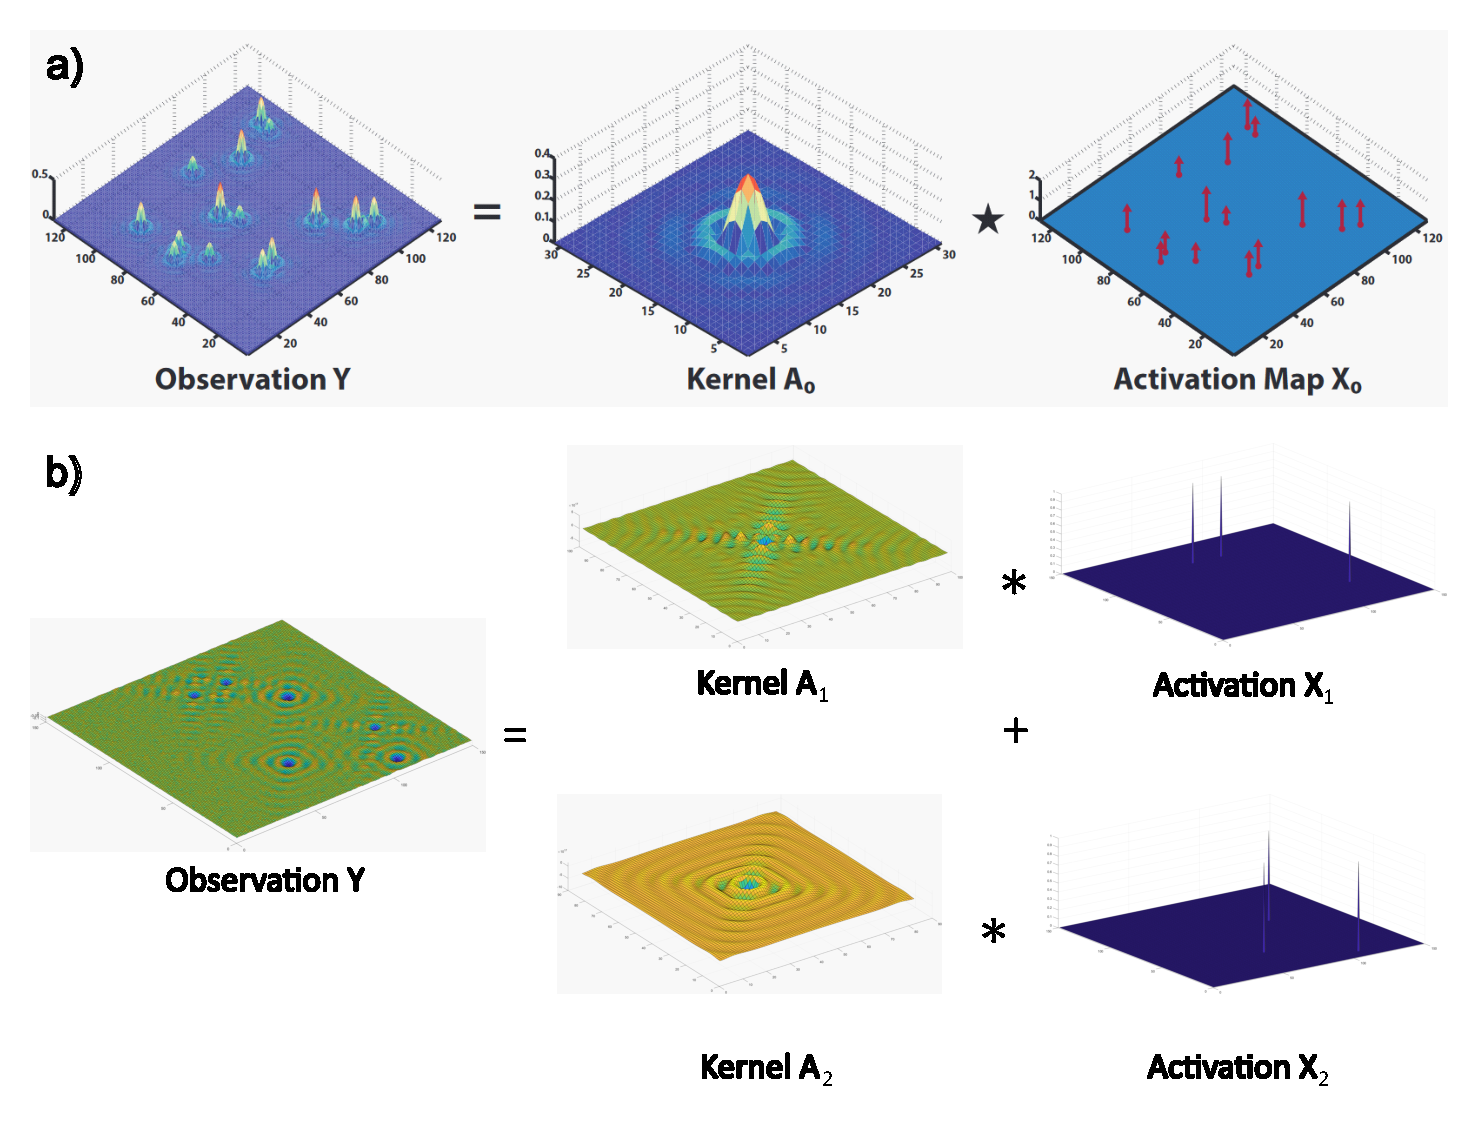
\includegraphics[width= \textwidth]{convolutional_model.pdf} 
	\centering
	\caption{Convolutional model of STM grid spectroscopy. a) Single defect convolutional model, introduced by Cheung et al to solve Sparse Blind Deconvolution(SBD) problem.\cite{cheungDictionaryLearningFouriertransform2020}. b) Multi-defect convolutional model, used to address \ac{MC-SBD} problem.}
	\label{fig:ch6_conv}
\end{figure}


\subsection{formulation of Multi-Channel Sparse Blind Deconvolution problem}
To understand the \ac{MC-SBD} problem, we need to first formulate its single-channel case --  the \ac{SBD} problem. Recall we can express the observed \ac{LDOS} $\delta\rho$ as the convolution between an individual QPI $\delta\rho_0$ and its defect location function $D(\mathbf{x})$ as: 
\begin{equation}
	\delta \rho(\mathbf{x}, \omega) = (\delta \rho_0 *D)(\mathbf{x}, \omega).
\end{equation}

\begin{figure}
	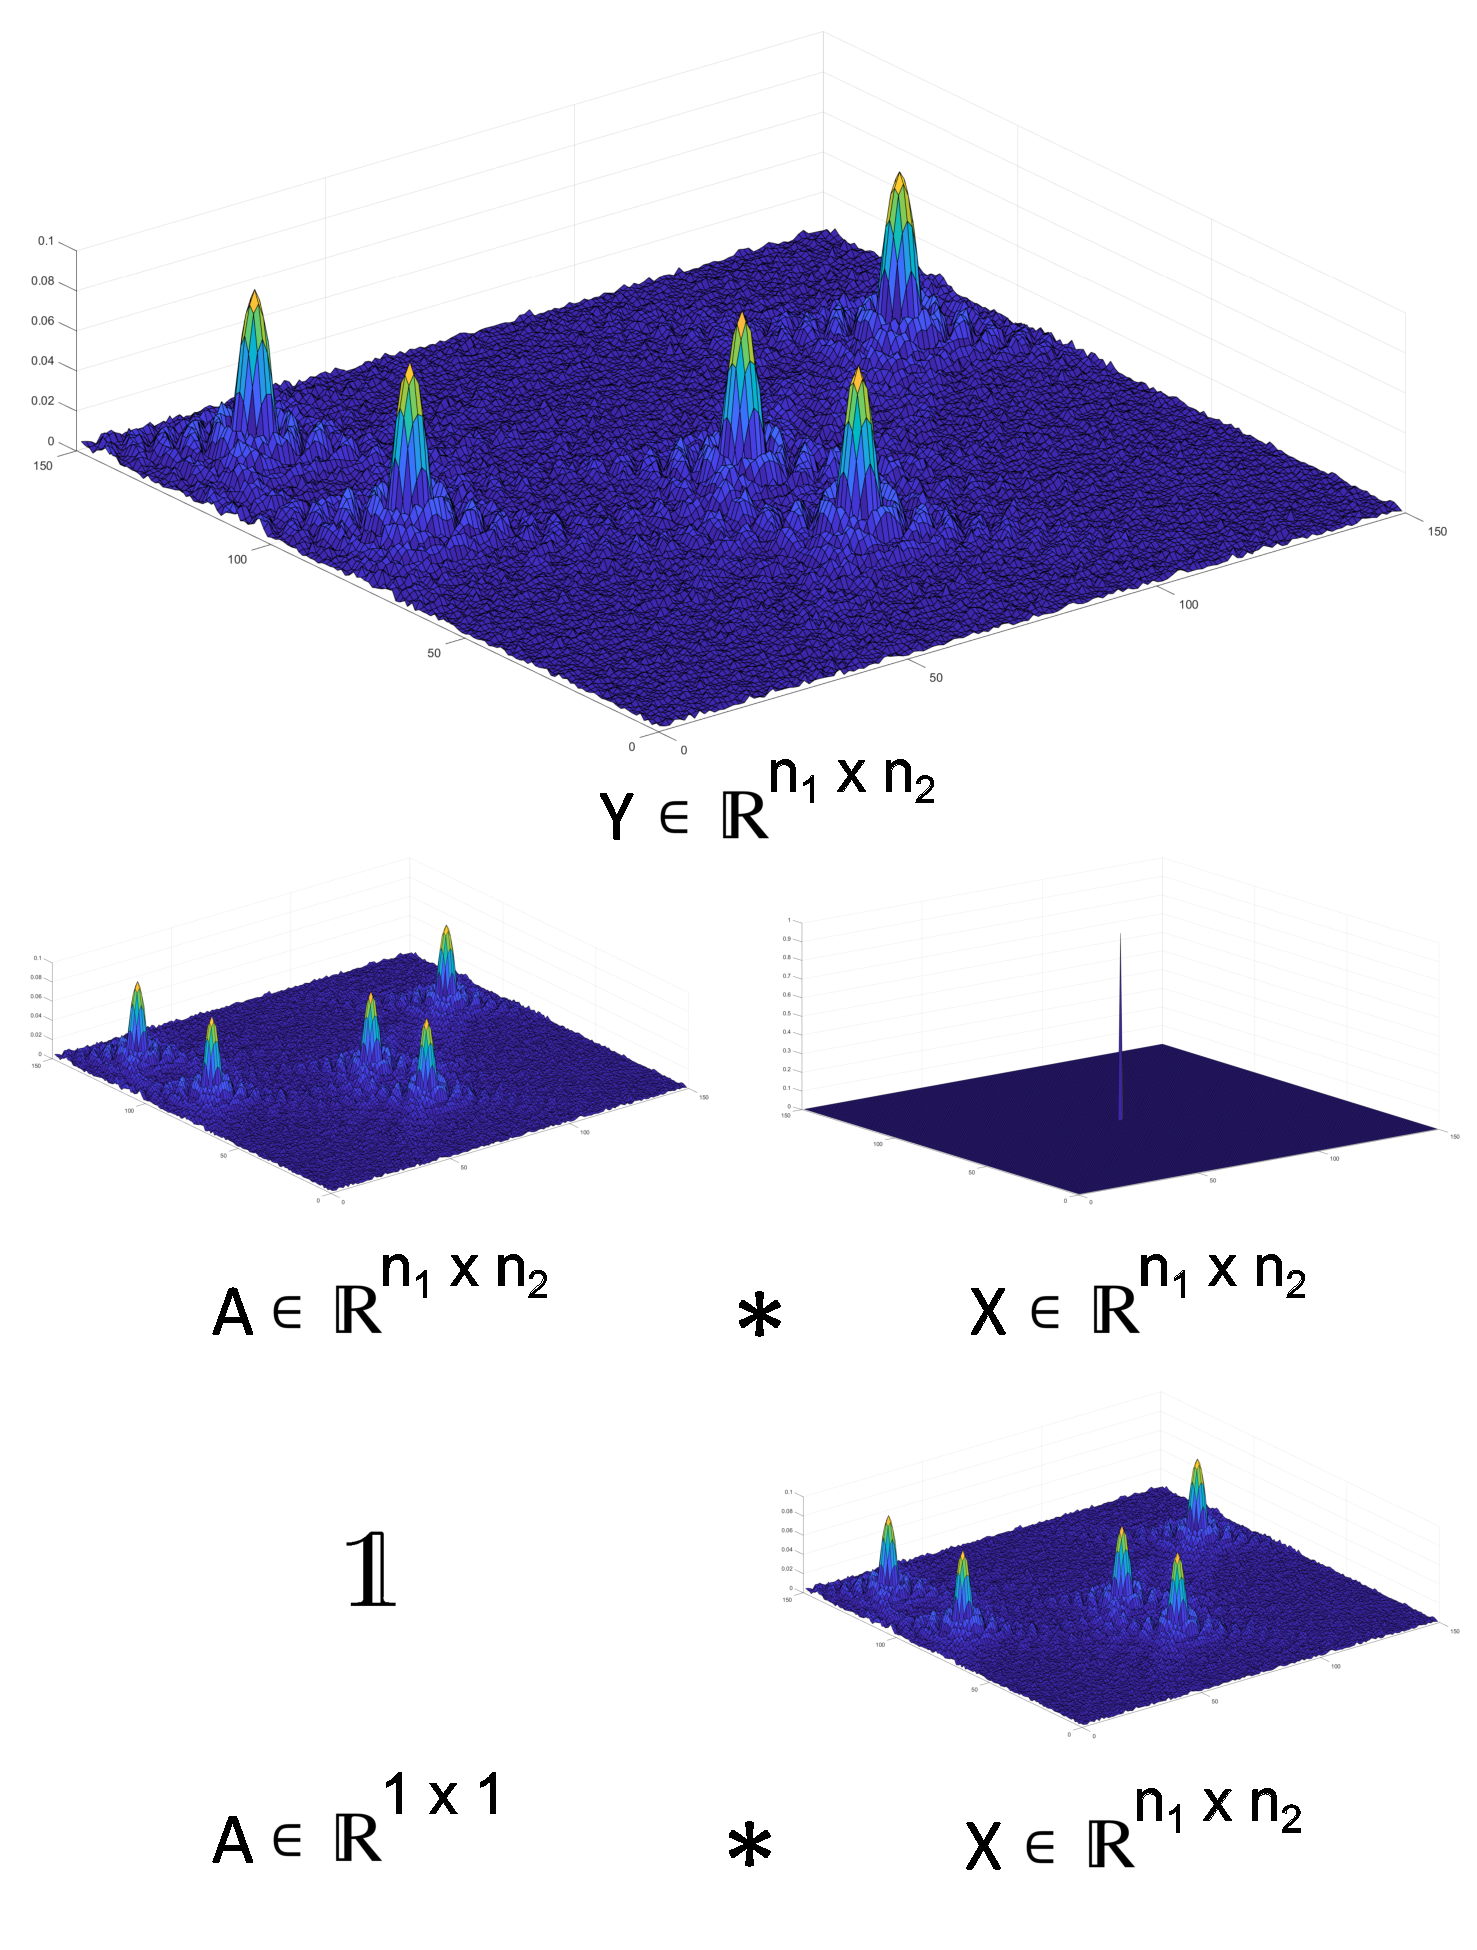
\includegraphics[width= \textwidth]{associativity.pdf} 
	\centering
	\caption{An extreme case illustrating associative symmetry of convolution. For any observation Y, there will always be two convolutions: one being we have a trivial activation, and all information is stored in the kernel with the same size as Y; The other is when we have a trivial scalar activation, and all information is stored in the activation}
	\label{fig:ch6_assoc}
\end{figure}

\noindent If we know the individual QPI pattern $\delta\rho_0$, and given the observed $\delta\rho$, we can inverse the convolution and get the defect location function $D(x)$; This is a deconvolution process. However, when $\delta\rho_0$ is unknown, it becomes a bilinear inverse problem known as \ac{BD}. However, as you may see, this is an ill-posed question, as there are many degenerate pairs of $(\delta\rho_0, D(\mathbf{x}))$ that could reconstruct the same observation. The reason behind these degeneracy is that the convolution is symmetric over several operations: 
\begin{itemize}
	\item \textbf{Translation Symmetry}: We obtain the same observation if we shift the kernel and activation map by an in-plane vector $\vec{\Delta}$ in the opposite direction. That is, given a translation operator $\operatorname{T}[f,\vec{\Delta}] \equiv f(\vec{x}+\vec{\Delta})$, we have:  
	\begin{equation}
		A_0 * X_0 = T[A_0,\vec{\Delta}] * T[X_0, -\vec{\Delta}].
	\end{equation}
	\item \textbf{Associative Symmetry}: Convolution operation is associative, meaning $(f * g) * h = f * (g *h)$, this has two implications, one is we have scaling symmetry: given $g = \alpha$, where $\alpha$ is a non-zero scalar, we have: 
	\begin{equation}
		A_0 * X_0 = (\frac{1}{\alpha})A_0*\alpha X_0.
	\end{equation}
	Another less trivial implication is we can have information leak between the kernel and the activation; That is, given $A_0 = A_0^L * A_0^R$ and $X_0= X_0^L * X_0^R$, where we express the kernel and the activation as convolutions, we have: 
	\begin{equation}
		A_0 * X_0 = (A_0^L * A_0^R * X_0^L) * X_0^R = A_0^L * (A_0^R * X_0^L * X_0^R).
	\end{equation}
	We can illustrate this with an extreme case shown in \ref{fig:ch6_assoc}. Given observation Y, two deconvolutional solutions are guaranteed by the associative symmetry, one is when the kernel resembles the observation and activation map is a delta function centered at the image origin, another is when all information leaked to the activation, and we are left with a trivial scalar kernel. While these extreme cases are not differentiable by the machine, they may seem absurd to us human; This is because we possess some intrinsic assumptions about the structure of both the kernel and the activation. By structuring our assumptions into rigorous formulations, we can indeed turn this ill-posed \ac{BD} problem well-posed. 
	
\end{itemize}



To break these symmetries and thus the corresponding degeneracy is crucial for a robust and reliable reconstruction. common approaches to break the symmetries including setting constrains to the manifold and introducing asymmetries to the cost function. For example,  enforcing A to stay in a hypersphere manifold $S = \{A \in \mathbb{R}^{m_1 \times m_2}: \vert\vert A \vert \vert_{F}= 1\}$, we can break the scaling symmetry except for the case when $\alpha = -1$. Additionally, the translation symmetry can be addressed by realizing the decaying nature for a QPI pattern, that is, the intensity near the edge of a kernel should approach zero; However, this restrain is weaker for kernels with larger size; this is illustrated in Figure.\ref{fig:ch6_t&s}, a) is the ground truth QPI pattern, it satisfy the constrain we set as the edge intensity naturally approaches zero due to the decay. We can then pad around a) with zeros to get a new kernel like b), note that this will still satisfy our constrains; We can pad it differently as shown in c) and d), thus recreating the degeneracy due to the translation symmetry. For this reason, we will see later that setting a proper spatial kernel size is crucial for our algorithm. 

Introducing asymmetries in the cost function is another important implementation, it is hard to visualize with problems in higher dimensions, we thus illustrate this with an example in 3D shown in Figure \ref{fig:ch6_reg}. Given potential energy $E_1 = sin(3x)\cdot cos(3x)$ with multiple local minimums, we can introducing a radial term $\lambda_r(x^2 + y^2$) to bias the local minimums closer to the origin, we can further tune the strength of the radial bias with $\lambda_r$ and set up a favorable energy landscape. This additional bias term is referred as a regularizar in the field of optimization, by assigning a proper regularizar to the cost function, we can turn the initially non-convex landscape to a more convex landscape, allowing a more stable and robust optimization. In our case, we will address the non-trivial associative symmetry by introducing a sparsity regularizar. 

\begin{figure}
	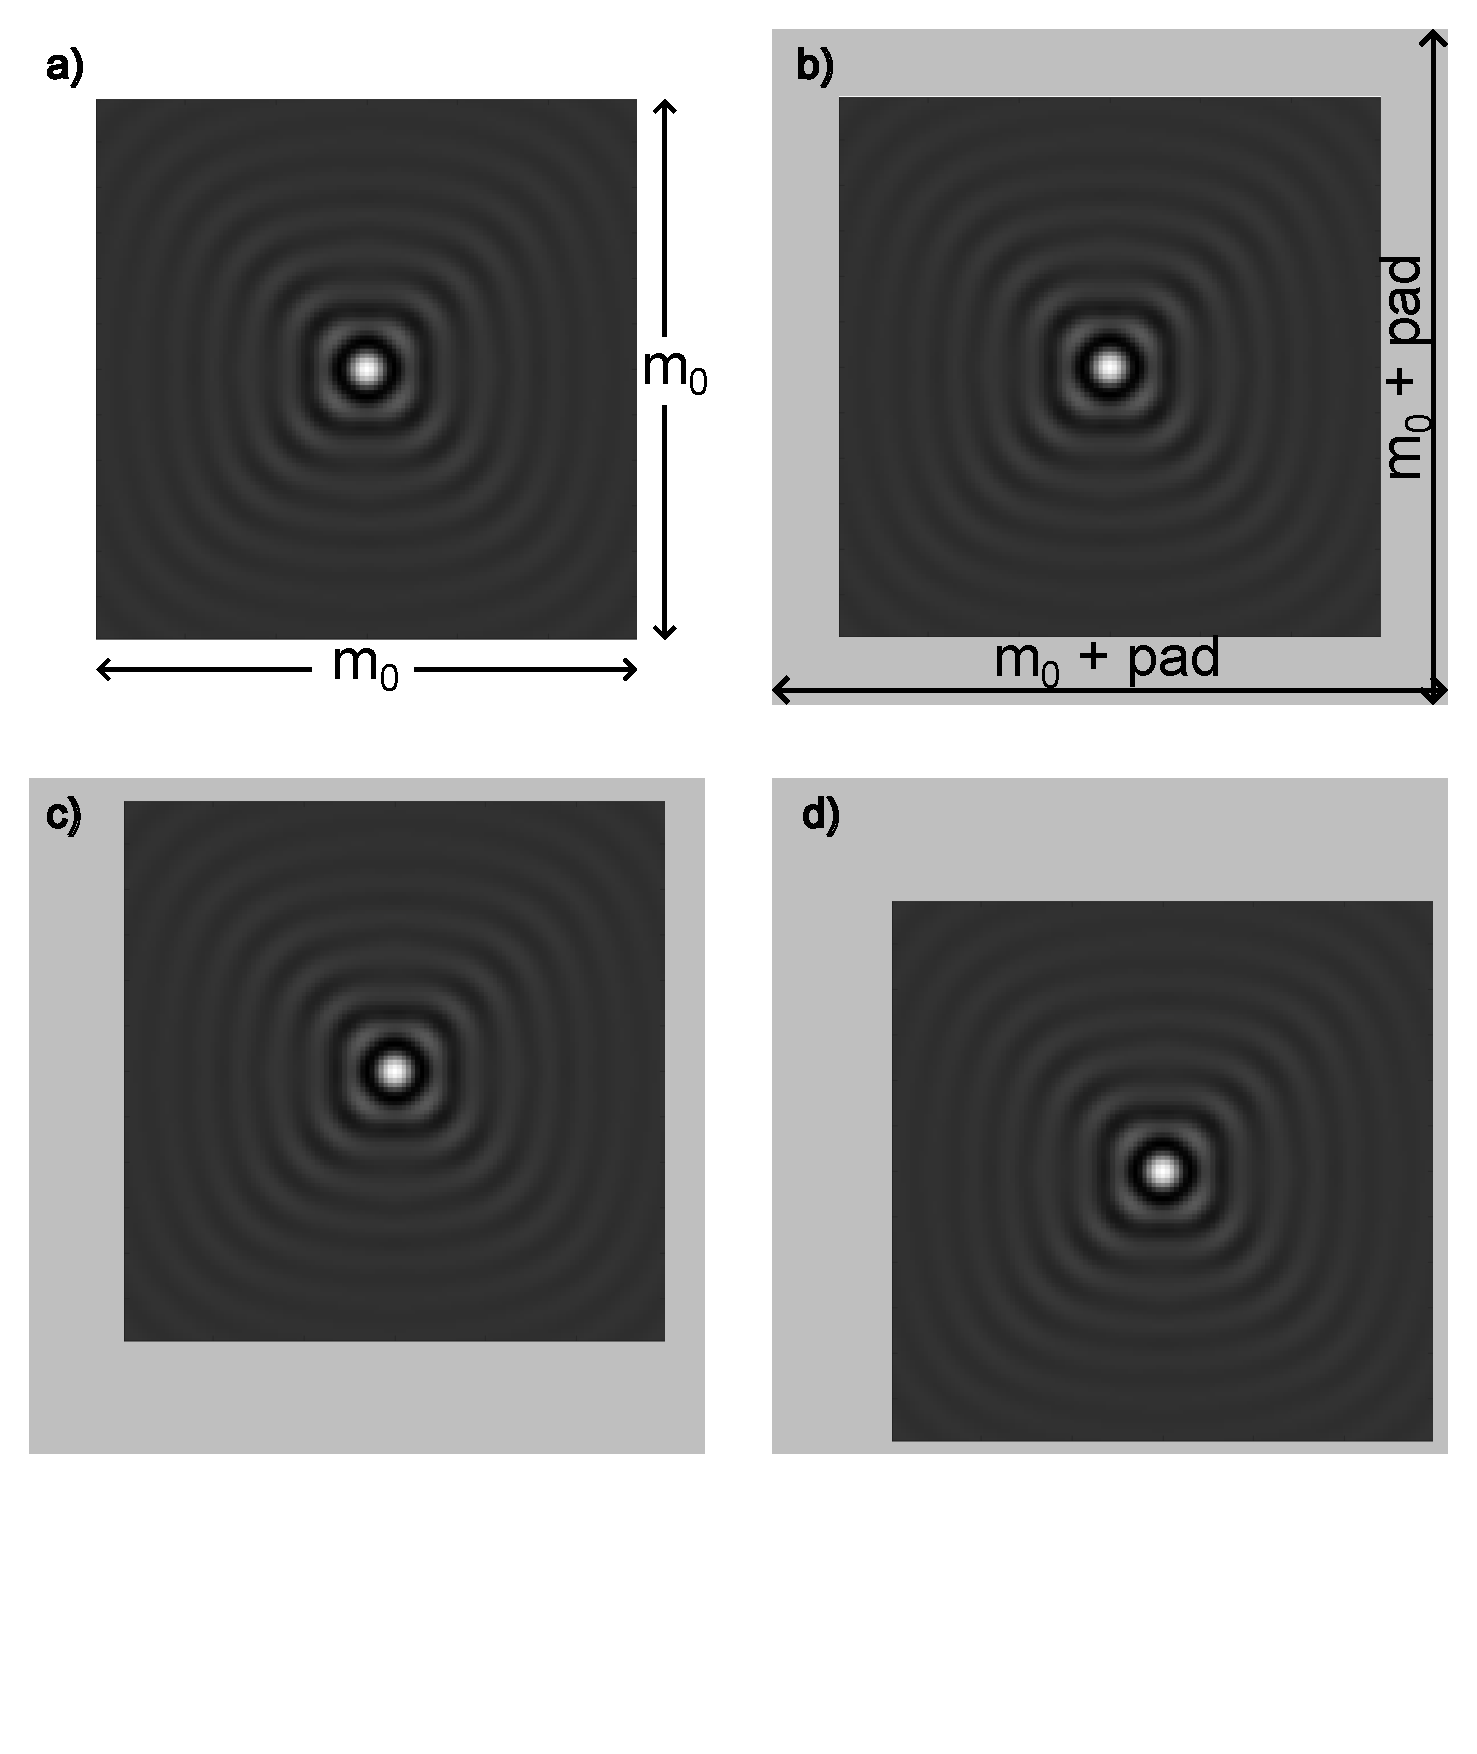
\includegraphics[width= \textwidth]{truncate and shift.pdf} 
	\centering
	\caption{Degeneracy caused by large kernel size. Given the ground truth QPI pattern (a) of size $m_0 \times m_0$, which naturally decays to near-zero intensity at the edges (or to the noise level in practical cases), this represents the ideal kernel we aim to reconstruct. However, ambiguity arises when constructing alternative kernels, such as in (b)–(d), by padding the ideal kernel with noise while preserving the vanishing edge condition. As the kernel size increases, the space of such degenerate solutions also grows, making the inverse problem increasingly ill-posed.}
	\label{fig:ch6_t&s}
\end{figure}

\begin{figure}
	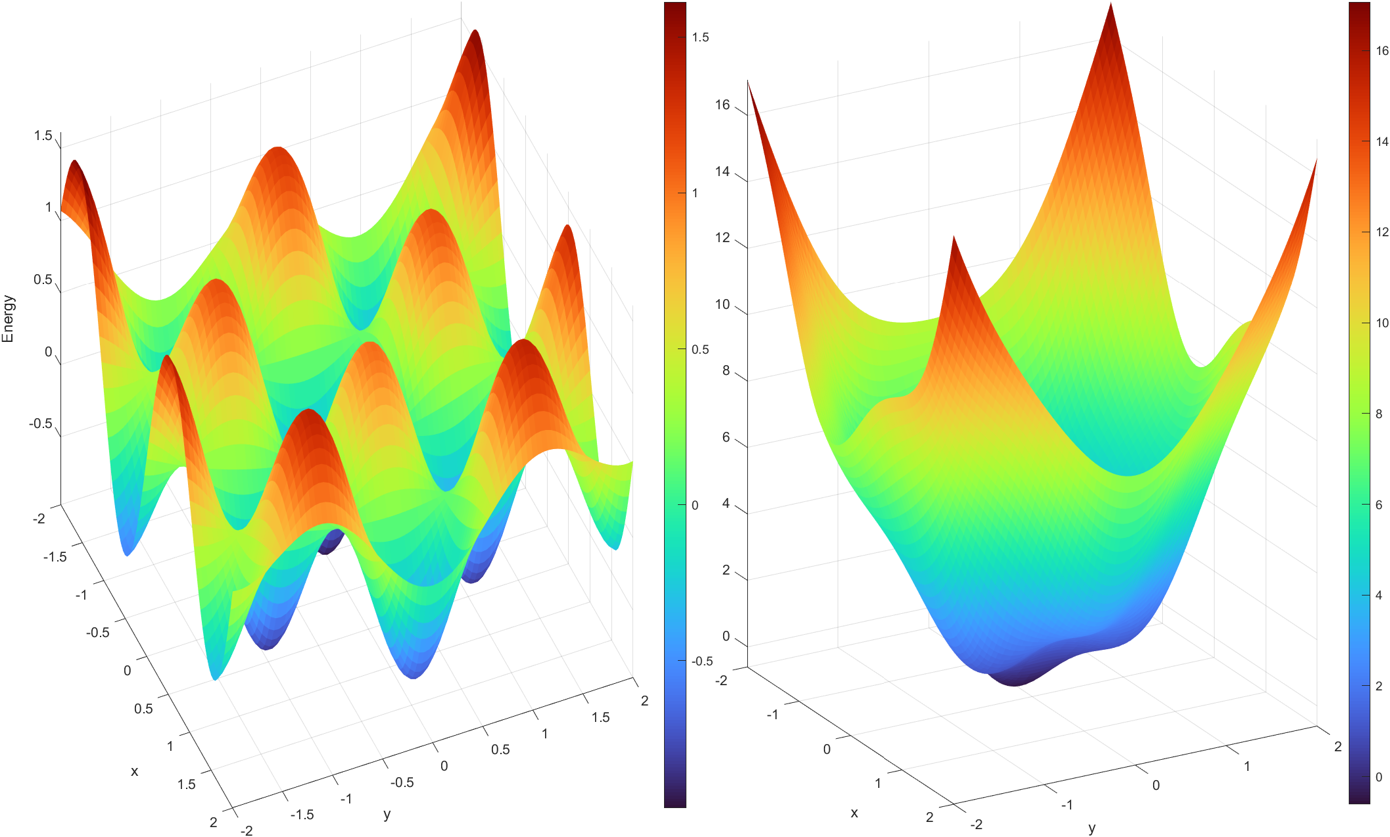
\includegraphics[width= \textwidth]{energy_reg.png} 
	\centering
	\caption{A low-dimension schematic showing how regularizar can make an initial non-convex problem convex. Left is the energy landscape created by $E_1 = sin(3x)\cdot cos(3x)$, this landscape is periodic in both spatial directions; Minimizing the energy is non-convex and ill-posed. However, if we add a regularizer $\phi_r \equiv \lambda_r(x^2 + y^2)$; with proper $\lambda$, this radial term will make $E_2 = E_1 + \phi_r$ convex. Right is an example of $E_2$ when we take $\lambda=2$.}
	\label{fig:ch6_reg}
\end{figure}

\subsubsection{The role of sparsity}
The sparsity regularizar acts on the activation map, by definition, an activation map $X_0$ is sparse when most of its entries are zero. Intuitively, we can define the regularizar to be proportional to $\left\lVert X\right\rVert_0$ -- X's $l_0$-norm, which is equal to the number of non-zero elements in $X$; However, $l_0$-norm is discrete and makes the cost function lost its continuity, which is harmful for the optimization process. We therefore replace $\left\lVert X\right\rVert_0$ with the $l_1$-norm $\left\lVert X\right\rVert_1 = \sum_{i=1}^{n}\vert x_i \vert$. We thus want to find $A_0$ and $X_0$ that minimize cost function $\phi_{\lambda}$:
\begin{equation}
	\phi_{\lambda} = \frac{1}{2}\left\lVert A_0 * X_0 - Y \right\rVert^2_F + \lambda \cdot \left\lVert X\right\rVert_1;
\end{equation}
\noindent The first term represent the data fidelity, where $\left\lVert \cdot\right\rVert_F$ represent the \textit{Frobenius norm}: 
\[
\left\lVert A \right\rVert_F = \sqrt{ \sum_{i=1}^{m} \sum_{j=1}^{n} |a_{ij}|^2 };
\] 
\noindent And $\lambda$ is a tunable parameter that we can set to vary the strength of the regularizer; Although bigger $\lambda$ normally results in a more convex problem, it can also overweight the data fidelity term and thus makes the result undesirable, a suitable range of $\lambda$ can be explored and tested in the practical runs. It is also worth noticing that in practice, even with an ideal $\lambda$, there may still be local minimums, making the problem non-convex globally, therefore, a good initial guess is usually required, especially for more challenging cases with multiple defects. 

We should discuss the validity of the sparse requirement for activation map. Recall that in our case, activation map $X$ represent the defect location map $D$, and the non-zero entries in the defect location map indicate the presence of a defect in the scan. Thus, lower defect concentration justifies the sparse requirement better. We can estimate a quantitative line of defect concentration where the sparse requirement could breakdown: Typically, a grid map takes a spatial linear resolution of 2-3 pixels per unit cell, for a square grid with the same linear resolution on each side, we have $\approx 10$ sampling points for a given unit cell. Note that the sparse requirement state that number of defects $N_d$ being much smaller than the sampling point $N_s = n_1 \times n_2$, say $N_d < \frac{N_s}{100}$, we get a cutoff defect concentration of $N_d^{cutoff} \approx 0.1$ per unit cell. This is a large defect concentration, moreover, this is the requirement not for the total defect concentration, but for a single type of defect; Thus, in most cases, it is safe to assume we satisfy the sparse requirement. However, dense defect cases can still break the assumption, and we will see in the later chapter that the algorithm's performance drops in the dense defect regime. 

\subsubsection{Complexity in Multi-Channel SBD}
We use the sparse nature of activation map to turn the bilinear Blind-Deconvolution problem into a better-posed Sparse Blind-Deconvolution problem. However, to address demixing problem, we need to encode multiple defect types into the algorithm formulation, this introduces extra level of complexity. 

First, multiple channels increases the dimension of the manifold, thus making the optimization process more computationally expensive. Another key source of complexity is the additional symmetries introduced with multi-channel, we illustrate these additional symmetries with a simplified 2-defect-type case, with the ground truth kernel and activation indicated with a superscript $gt$: 
\begin{equation*}
	Y = A_1^{gt}*X_1^{gt} + A_2^{gt}*X_2^{gt}
\end{equation*} 

\begin{itemize}
	\item \textbf{Linear Mixing Equivalence}: This equivalence roots from the distributive rule of the convolution: $(f_1+f_2)*g = f_1*g + f_2*g$. Given: 
	\begin{align*}
		A_1 &= aA_1^{gt}+bA_2^{gt}, \\
		A_2 &= cA_1^{gt}+dA_2^{gt}, \\
		X_1 &= a'X_1^{gt}+b'X_2^{gt}, \\
		X_2 &= c'X_1^{gt}+d'X_2^{gt}; \\
	\end{align*}
	We have: 
	\begin{align*}
		A_1*X_1 +A_2*X_2= (aa'+cc') A_1^{gt}*X_1^{gt}+ (bb'+dd')A_2^{gt}*X_2^{gt} \\+ (ab'+cd') A_1^{gt}*X_2^{gt} +(ba'+dc') A_2^{gt}*X_1^{gt},
	\end{align*}
	To ensure $A_1*X_1 +A_2*X_2 = A_1^{gt}*X_1^{gt} + A_2^{gt}*X_2^{gt}$, we meed to consider two cases, the easier case is when we have two very distinctive ground truth kernels and the off-diagonal terms are linearly-independent from the diagonal terms. Thus, we want to eliminate the $A_1^{gt}*X_2^{gt}$ and $A_2^{gt}*X_1^{gt}$ terms, and we need to satisfy:
	 \begin{align*}
	 	ab'+cd'&= ba' + dc' = 0, \\
	 	aa'+cc'&= bb' + dd' = 1; \\
	 \end{align*}
	 With 4 equations and 8 unknowns, we are left with 4 degrees of freedom within the degeneracy space. Note that this is with 2 types of defects, with n types of defects, the degeneracy space will expand with n square. In the case of similar ground truth kernels, we might have cross-talks between the off-diagonal terms and diagonal terms; This leaves us with a even larger degeneracy space. 
\end{itemize}

In real STM studies, materials usually present more types of defects. As illustrated in Figure \ref{fig:ch6_defect} a), it is an STM topography taken on ZrSiTe, there are 4 distinct types of defects circled in red, moreover, we have the same type of defect but rotated 90 degrees circled in yellow. It is not uncommon to see rotated defects, as defect formation follows the lattice symmetry; The rotation of same type of defect can be better illustrated in PtSn$_4$ as shown in b), where 4 croissant defects at 4 orientations are circled in yellow. In \ac{MC-SBD}, each orientations of the croissant defects will be treated as a new type of defect, therefore, even with only 1 type of defect, we might need to use multiple kernels; This further shows the challenging nature of the problem, as well as the necessity to extend the single defect \ac{SBD} algorithm to \ac{MC-SBD}.

\begin{figure}
	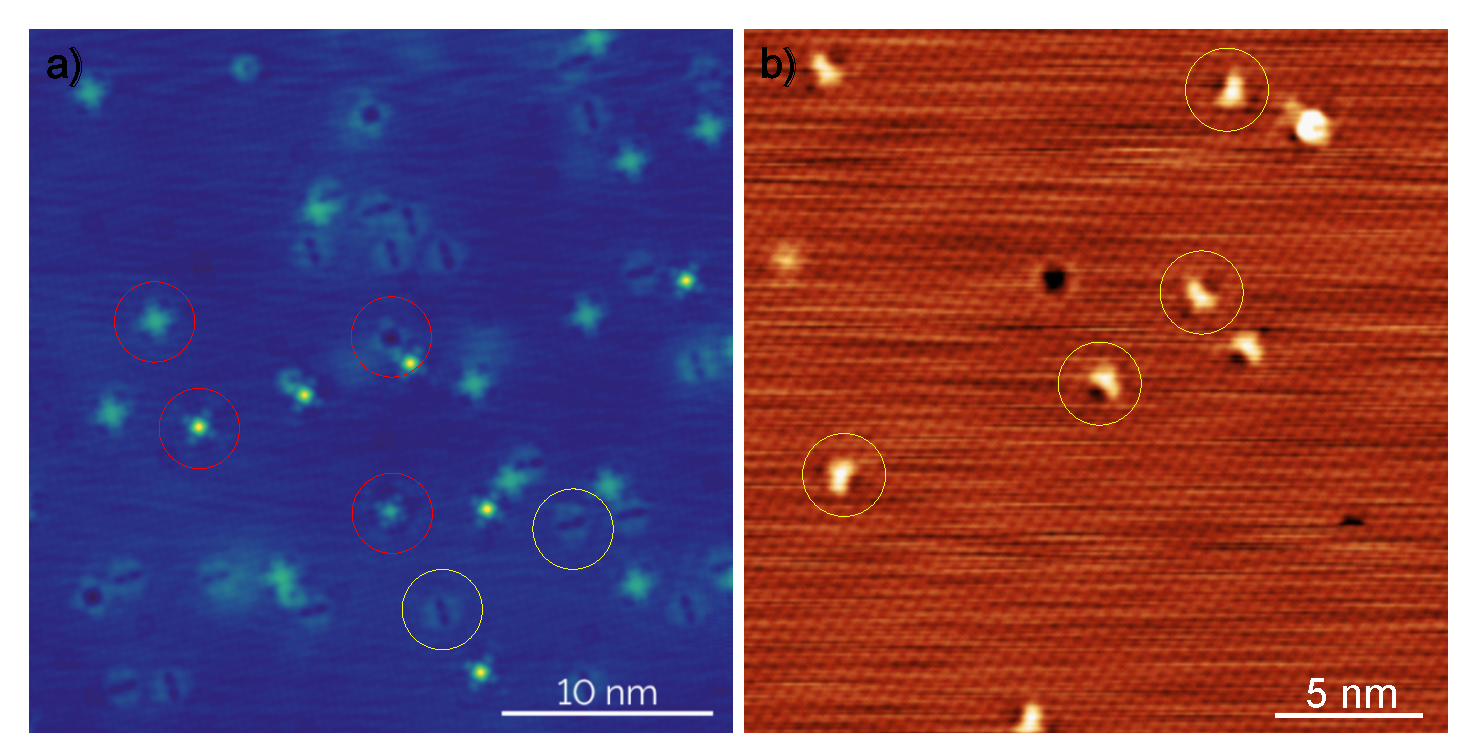
\includegraphics[width= \textwidth]{defect_types.pdf} 
	\centering
	\caption{}
	\label{fig:ch6_defect}
\end{figure}